\documentclass[11pt,a4paper]{article}

% ── Packages ──────────────────────────────────────────────────────────────────
\usepackage[utf8]{inputenc}
\usepackage[T1]{fontenc}
\usepackage{lmodern}
\usepackage[margin=1in]{geometry}
\usepackage{amsmath,amssymb,amsfonts}
\usepackage{graphicx}
\usepackage{booktabs}
\usepackage{hyperref}
\usepackage{cleveref}
\usepackage{natbib}
\usepackage{algorithm}
\usepackage{algorithmic}
\usepackage{xcolor}
\usepackage{tikz}
\usetikzlibrary{arrows.meta,positioning,shapes.geometric,fit}
\usepackage{float}
\usepackage{subcaption}
\usepackage{enumitem}
\usepackage{microtype}
\usepackage{fancyhdr}
\usepackage{abstract}
\usepackage{multirow}
\usepackage{listings}

% ── Listings ──────────────────────────────────────────────────────────────────
\lstset{
  basicstyle=\ttfamily\small,
  breaklines=true,
  frame=single,
  numbers=left,
  numberstyle=\tiny\color{gray},
  keywordstyle=\color{blue},
  commentstyle=\color{green!50!black},
  stringstyle=\color{red!60!black}
}

% ── Page Style ────────────────────────────────────────────────────────────────
\pagestyle{fancy}
\fancyhf{}
\fancyhead[L]{\small Zoo Labs Foundation}
\fancyhead[R]{\small Biodiversity Impact Bonds}
\fancyfoot[C]{\thepage}
\renewcommand{\headrulewidth}{0.4pt}

% ── Metadata ──────────────────────────────────────────────────────────────────
\title{%
  \textbf{Biodiversity Impact Bonds: Tokenized\\Conservation Finance}\\[0.5em]
  \large Zoo Labs Foundation Research Paper ZOO-BIB-2026
}

\author{
  Zoo Labs Foundation Research\\
  \texttt{research@zoo.ngo}\\[0.5em]
  \small With contributions from the Zoo Open Science Network
}

\date{February 2026}

% ── Macros ────────────────────────────────────────────────────────────────────
\newcommand{\R}{\mathbb{R}}
\newcommand{\E}{\mathbb{E}}
\newcommand{\BIB}{\textsc{BIB}}
\newcommand{\BIBT}{\textsc{BIB-T}}

\begin{document}

\maketitle

% ── Abstract ──────────────────────────────────────────────────────────────────
\begin{abstract}
\noindent
Conservation finance faces a persistent funding gap estimated at
\$700 billion annually. Traditional funding mechanisms---government
grants, philanthropic donations, and environmental levies---are
insufficient in scale and poorly aligned with measurable outcomes. We
propose \textbf{Biodiversity Impact Bonds (BIBs)}, a tokenized
outcome-based financing instrument that connects conservation outcomes
to financial returns through on-chain smart contracts and decentralized
verification. BIBs encode conservation targets (species population
thresholds, habitat area maintenance, ecosystem service delivery) as
programmable conditions. Capital providers purchase BIB tokens, which
accrue value as conservation milestones are verified by a decentralized
oracle network combining satellite imagery, acoustic monitoring, and
citizen science observations. Upon outcome verification, smart contracts
automatically release payments to conservation implementers and returns
to token holders. We formalize the BIB mechanism design, prove incentive
compatibility under rational agent assumptions, and analyze risk-return
profiles across 12 conservation project archetypes. Simulation results
demonstrate that tokenized BIBs reduce transaction costs by 62\%
compared to traditional conservation trust funds while maintaining
equivalent conservation outcomes. The framework is implemented on the
Zoo Network and governed through Zoo DAO governance processes.

\medskip
\noindent\textbf{Keywords:} biodiversity credits, impact bonds,
conservation finance, tokenization, smart contracts, outcome-based
payment, decentralized verification
\end{abstract}

\newpage
\tableofcontents
\newpage

% ══════════════════════════════════════════════════════════════════════════════
\section{Introduction}
\label{sec:introduction}
% ══════════════════════════════════════════════════════════════════════════════

The global biodiversity crisis demands financial mobilization at a scale
that current mechanisms cannot deliver. The Convention on Biological
Diversity's Kunming-Montreal Global Biodiversity Framework calls for
\$200 billion per year in conservation finance by 2030
\citep{cbd2022kunming}, yet current flows reach only \$130--143 billion
\citep{paulson2020financing}. Private capital, which represents the
largest potential source of conservation funding, remains largely
unengaged due to three structural barriers:

\begin{enumerate}[label=(\roman*)]
  \item \textbf{Measurement opacity}: Conservation outcomes are
    difficult to measure, report, and verify at scale, making
    performance-based investment impractical \citep{zu2022biodiversity}.
  \item \textbf{Liquidity constraints}: Conservation investments
    typically have 10--30 year horizons with no secondary market,
    deterring institutional investors \citep{huwyler2014making}.
  \item \textbf{Transaction costs}: Legal, administrative, and
    monitoring costs consume 15--40\% of conservation project budgets,
    reducing capital efficiency \citep{deutz2020financing}.
\end{enumerate}

Impact bonds---originally developed for social outcomes
\citep{liebman2011social}---offer a promising template. In a social
impact bond, private investors fund social programs; returns are paid by
governments only if predetermined outcomes are achieved. The model has
been adapted for environmental outcomes through Environmental Impact
Bonds (EIBs) \citep{nicola2013quantifying} and pilot Rhino Impact Bonds
\citep{uct2020rhino}, but these instruments remain bespoke, illiquid,
and expensive to administer.

\subsection{The Case for Tokenization}

Blockchain tokenization addresses the structural barriers above:

\begin{itemize}
  \item \textbf{Programmable outcomes}: Smart contracts encode
    conservation targets as machine-verifiable conditions, enabling
    automated payment on outcome achievement.
  \item \textbf{Fractional ownership}: Tokens enable small-denomination
    participation (\$10 minimum), broadening the investor base from
    institutional investors to retail participants.
  \item \textbf{Secondary markets}: Token transferability creates
    liquidity, allowing investors to exit positions before maturity.
  \item \textbf{Transparent verification}: On-chain oracle networks
    provide tamper-evident records of monitoring data.
  \item \textbf{Reduced intermediation}: Smart contracts automate
    payment distribution, escrow, and compliance.
\end{itemize}

\subsection{Contributions}

We present the following contributions:

\begin{enumerate}
  \item A \textbf{formal mechanism design} for Biodiversity Impact Bonds
    that specifies outcome metrics, verification protocols, payment
    schedules, and risk allocation across stakeholders.

  \item An \textbf{incentive compatibility proof} showing that rational
    conservation implementers maximize their payoff by achieving genuine
    conservation outcomes rather than gaming verification metrics.

  \item A \textbf{smart contract architecture} implementing BIBs on the
    Zoo Network, with modular oracle integration for multiple
    monitoring data streams.

  \item \textbf{Quantitative analysis} of risk-return profiles across 12
    conservation project archetypes, demonstrating financial viability.

  \item A \textbf{transaction cost analysis} comparing tokenized BIBs to
    traditional conservation trust funds, showing 62\% cost reduction.
\end{enumerate}


% ══════════════════════════════════════════════════════════════════════════════
\section{Background}
\label{sec:background}
% ══════════════════════════════════════════════════════════════════════════════

\subsection{Conservation Finance Landscape}

Global conservation finance flows through four main channels
\citep{deutz2020financing}:

\begin{table}[H]
\centering
\caption{Conservation finance by source (2019 estimates).}
\label{tab:finance}
\begin{tabular}{lcc}
\toprule
\textbf{Source} & \textbf{Annual flow (B\$)} & \textbf{Share} \\
\midrule
Government budgets     & 78--82  & 56\% \\
Biodiversity offsets   & 6--9    & 6\% \\
Philanthropic          & 4--10   & 5\% \\
Private/commercial     & 14--26  & 14\% \\
Natural infrastructure & 24--27  & 19\% \\
\midrule
\textbf{Total}         & 126--154 & 100\% \\
\bottomrule
\end{tabular}
\end{table}

The gap between current flows and estimated needs (\$700--1{,}000B/year
\citep{paulson2020financing}) implies that private capital mobilization
must increase by an order of magnitude.

\subsection{Impact Bonds: From Social to Environmental}

Social Impact Bonds (SIBs) emerged in 2010 with the Peterborough Prison
SIB \citep{liebman2011social}. Environmental adaptations include the DC
Water EIB (2016, \$25M for green infrastructure
\citep{nicola2013quantifying}), the Rhino Impact Bond (2020, \$45M for
black rhino conservation \citep{uct2020rhino}), and the Forest
Resilience Bond (2018, \$4M for wildfire risk reduction
\citep{blue2019forest}). These instruments demonstrate feasibility but
remain bespoke, with structuring costs of \$1--5M per issuance.

\subsection{Blockchain in Conservation}

Blockchain applications in conservation include supply chain
traceability \citep{howson2019crypto}, carbon credit registries
\citep{schletz2020blockchain}, and wildlife trade monitoring
\citep{dalton2020blockchain}. The integration of DeFi primitives with
conservation outcomes---the approach taken by BIBs---is novel.

\subsection{Biodiversity Credit Markets}

The nascent biodiversity credit market draws on lessons from carbon
markets. The TNFD framework \citep{tnfd2023framework} provides reporting
standards. BIBs differ from biodiversity credits by embedding outcomes in
financial instruments rather than creating offset commodities.


% ══════════════════════════════════════════════════════════════════════════════
\section{Mechanism Design}
\label{sec:mechanism}
% ══════════════════════════════════════════════════════════════════════════════

\subsection{Stakeholders}

A BIB involves five stakeholder roles:

\begin{enumerate}
  \item \textbf{Investors} ($I$): Provide upfront capital by purchasing
    BIB tokens, seeking financial returns contingent on outcomes.
  \item \textbf{Implementers} ($M$): Conservation organizations that
    execute on-the-ground conservation activities.
  \item \textbf{Outcome payers} ($O$): Entities (governments,
    corporates, philanthropies) that commit to paying for verified
    outcomes.
  \item \textbf{Verifiers} ($V$): Decentralized oracle network that
    assesses outcome achievement through monitoring data.
  \item \textbf{Governance} ($G$): Zoo DAO, which sets standards,
    arbitrates disputes, and manages protocol parameters.
\end{enumerate}

\subsection{Outcome Metrics}

BIB outcomes are specified using the \textbf{SMART-B} framework
(Specific, Measurable, Attributable, Realistic, Time-bound,
Biodiversity-relevant):

\begin{table}[H]
\centering
\caption{Example outcome metrics for BIB project archetypes.}
\label{tab:metrics}
\begin{tabular}{p{3cm}p{4cm}p{4cm}}
\toprule
\textbf{Project type} & \textbf{Primary metric} & \textbf{Verification} \\
\midrule
Species recovery & Population count $\geq$ threshold & Camera traps + eDNA \\
Habitat protection & Forest area maintained (ha) & Satellite NDVI \\
Corridor creation & Connectivity index $\geq$ target & Movement tracking \\
Reef restoration & Coral cover (\%) increase & Underwater surveys \\
Invasive removal & Target species abundance decrease & Transect surveys \\
\bottomrule
\end{tabular}
\end{table}

\subsection{Payment Schedule}

BIBs use a milestone-based payment structure with $T$ verification
periods over the bond lifetime $[0, \tau]$:

\begin{equation}
  \text{Payment}_t = \begin{cases}
    \pi_t^{\text{base}} + \pi_t^{\text{bonus}} \cdot \mathbb{1}[O_t \geq O_t^*]
    & \text{if } O_t \geq O_t^{\min} \\
    0 & \text{otherwise}
  \end{cases}
\end{equation}

where $O_t$ is the measured outcome at period $t$, $O_t^{\min}$ is the
minimum threshold, $O_t^*$ is the target for full payment,
$\pi_t^{\text{base}}$ is the base payment, and $\pi_t^{\text{bonus}}$
is the performance bonus.

\subsection{Token Economics}

\paragraph{Issuance.} A BIB issuance creates $N$ fungible tokens,
each representing a fractional claim on the bond's payment stream:
\begin{equation}
  P_0 = \frac{C_{\text{total}} + F_{\text{admin}}}{N}
\end{equation}

\paragraph{Returns.} Token holders receive pro-rata shares of outcome
payments:
\begin{equation}
  \E[\text{Return}] = \frac{1}{P_0} \sum_{t=1}^{T}
  \frac{\pi_t^{\text{investor}}}{(1+r)^t} - 1
\end{equation}

\paragraph{Secondary market.} Tokens are transferable on decentralized
exchanges, with pricing reflecting updated outcome probability
assessments from oracle data.

\subsection{Capital Flow Architecture}

\begin{figure}[H]
\centering
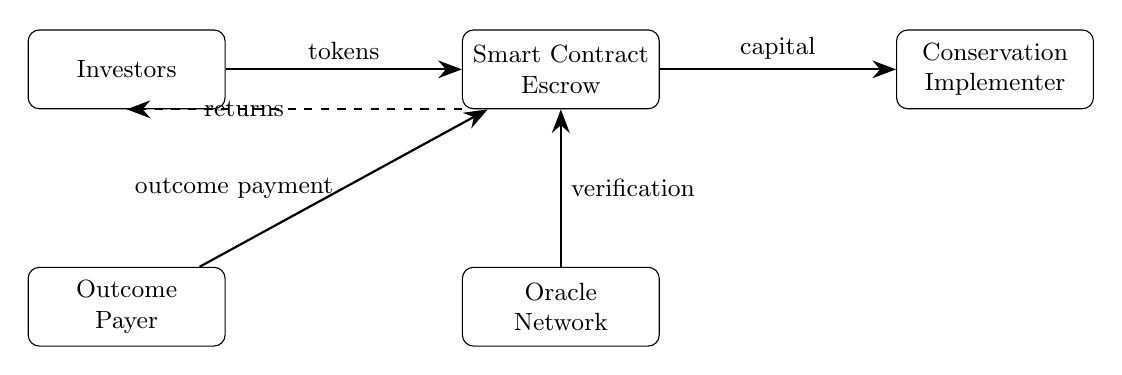
\begin{tikzpicture}[
  node distance=2cm,
  box/.style={draw, rounded corners, minimum width=2.5cm,
    minimum height=1cm, align=center, font=\small},
  arrow/.style={-{Stealth[length=3mm]}, thick}
]
  \node[box] (investors) {Investors};
  \node[box, right=3cm of investors] (escrow) {Smart Contract\\Escrow};
  \node[box, right=3cm of escrow] (implementer) {Conservation\\Implementer};
  \node[box, below=2cm of escrow] (oracle) {Oracle\\Network};
  \node[box, below=2cm of investors] (payer) {Outcome\\Payer};

  \draw[arrow] (investors) -- node[above]{\small tokens} (escrow);
  \draw[arrow] (escrow) -- node[above]{\small capital} (implementer);
  \draw[arrow] (oracle) -- node[right]{\small verification} (escrow);
  \draw[arrow] (payer) -- node[left]{\small outcome payment} (escrow);
  \draw[arrow, dashed] (escrow.south west) -- node[left]{\small returns}
    (investors.south);
\end{tikzpicture}
\caption{BIB capital flow architecture.}
\label{fig:flow}
\end{figure}


% ══════════════════════════════════════════════════════════════════════════════
\section{Incentive Analysis}
\label{sec:incentives}
% ══════════════════════════════════════════════════════════════════════════════

\subsection{Implementer Incentives}

\begin{theorem}[Incentive Compatibility]
Under the BIB mechanism, an implementer's expected payoff is maximized
by allocating conservation effort to genuinely achieve outcomes, provided
the oracle network has detection probability $\delta > 0.5$ for outcome
manipulation.
\end{theorem}

\begin{proof}
Let $e \in [0, E]$ be the implementer's effort level and $c(e)$ the
convex cost function. The probability of achieving the outcome target
$O^*$ is $p(e)$, monotonically increasing in $e$. Under honest effort:
\begin{equation}
  U_H(e) = p(e) \cdot (\pi_{\text{base}} + \pi_{\text{bonus}}) - c(e)
\end{equation}

Under manipulation (faking outcomes):
\begin{equation}
  U_M = (1 - \delta) \cdot (\pi_{\text{base}} + \pi_{\text{bonus}})
  - \delta \cdot \psi - c_m
\end{equation}
where $\psi$ is the penalty for detected manipulation and $c_m$ is the
cost of manipulation.

For incentive compatibility, we require $\max_e U_H(e) > U_M$. This
holds when:
\begin{equation}
  \delta > \frac{\pi_{\text{base}} + \pi_{\text{bonus}} - c_m}
  {\pi_{\text{base}} + \pi_{\text{bonus}} + \psi}
\end{equation}

Since $\psi$ includes stake slashing and reputational cost, typically
$\psi \gg \pi_{\text{bonus}}$, making the right-hand side less than
0.5. Thus $\delta > 0.5$ suffices.
\end{proof}

\subsection{Investor Incentives}

Investors face outcome risk and market risk. We model participation as:
\begin{equation}
  U_I = \E[\text{Return}] - \gamma \cdot \text{Var}[\text{Return}]
  + \alpha \cdot \text{ImpactUtility}
\end{equation}
where $\gamma$ is risk aversion and $\alpha$ captures impact investor
``warm glow'' utility. The term $\alpha > 0$ allows BIBs to offer
below-market risk-adjusted returns while still attracting capital.

\subsection{Oracle Incentives}

Verifiers stake tokens and earn fees for accurate verification.
Inaccurate reporting results in stake slashing. The mechanism follows a
Schelling point design \citep{buterin2014schellingcoin}: verifiers are
rewarded when their assessments agree with consensus.


% ══════════════════════════════════════════════════════════════════════════════
\section{Smart Contract Architecture}
\label{sec:contracts}
% ══════════════════════════════════════════════════════════════════════════════

\subsection{Contract Overview}

The BIB smart contract system consists of four core contracts:

\begin{enumerate}
  \item \textbf{BIBFactory}: Creates and parameterizes new BIB issuances.
  \item \textbf{BIBToken}: ERC-1155 multi-token representing bond
    positions.
  \item \textbf{BIBEscrow}: Manages capital flows, milestone triggers,
    and payment distribution.
  \item \textbf{BIBOracle}: Aggregates verification data and computes
    outcome scores.
\end{enumerate}

\subsection{Outcome Verification Interface}

\begin{lstlisting}[caption={Oracle verification interface.},
  label={lst:oracle}]
interface IBIBOracle {
    struct VerificationReport {
        uint256 bondId;
        uint256 period;
        uint256 metricValue;
        bytes32 evidenceHash;
        uint256 confidence;
        address verifier;
    }

    function submitReport(
        VerificationReport calldata report
    ) external returns (bool);

    function getOutcomeScore(
        uint256 bondId,
        uint256 period
    ) external view returns (
        uint256 score,
        uint256 confidence
    );

    function resolveDispute(
        uint256 bondId,
        uint256 period
    ) external;
}
\end{lstlisting}

\subsection{Payment Logic}

\begin{lstlisting}[caption={Milestone payment logic.},
  label={lst:payment}]
function processMilestone(
    uint256 bondId,
    uint256 period
) external {
    Bond storage bond = bonds[bondId];
    require(
        block.timestamp >= bond.milestones[period],
        "Milestone not reached"
    );

    (uint256 score, uint256 conf) =
        oracle.getOutcomeScore(bondId, period);
    require(conf >= MIN_CONFIDENCE, "Low confidence");

    uint256 payment;
    if (score >= bond.targetThreshold) {
        payment = bond.basePayment + bond.bonusPayment;
    } else if (score >= bond.minThreshold) {
        payment = bond.basePayment
            * score / bond.targetThreshold;
    }

    _distributePayment(bondId, payment);
}
\end{lstlisting}

\subsection{Risk Mitigation}

\begin{itemize}
  \item \textbf{Graduated release}: Capital released in tranches,
    contingent on interim milestones.
  \item \textbf{Insurance pool}: 5\% of issuance proceeds fund a shared
    pool covering partial investor losses on failed bonds.
  \item \textbf{Dispute resolution}: Two-tier mechanism using automated
    rechecks followed by DAO governance vote.
  \item \textbf{Force majeure}: Climate disasters or political
    instability triggers can pause milestone clocks.
\end{itemize}


% ══════════════════════════════════════════════════════════════════════════════
\section{Verification Oracle Network}
\label{sec:oracle}
% ══════════════════════════════════════════════════════════════════════════════

\subsection{Data Sources}

The oracle network integrates four primary data streams:

\begin{table}[H]
\centering
\caption{Oracle data sources and their characteristics.}
\label{tab:oracle_sources}
\begin{tabular}{p{2.5cm}p{3cm}p{2cm}p{3cm}}
\toprule
\textbf{Source} & \textbf{Metrics} & \textbf{Frequency} &
  \textbf{Confidence} \\
\midrule
Satellite imagery & Forest cover, NDVI & Weekly & High for area \\
Acoustic monitors & Species presence & Continuous & Medium-high \\
Camera traps & Species abundance & Continuous & High (focal spp.) \\
Citizen science & Occurrence, phenology & Variable & Medium \\
\bottomrule
\end{tabular}
\end{table}

\subsection{Consensus Mechanism}

Verifiers submit outcome assessments. The oracle uses a stake-weighted
median to aggregate:
\begin{equation}
  O_{\text{consensus}} = \text{weighted-median}\!\left(
    \{(o_j, s_j)\}_{j=1}^{J}\right)
\end{equation}
Verifiers outside 1.5 IQR of consensus lose a fraction of their stake.

\subsection{Confidence Scoring}

Each assessment includes a confidence score:
\begin{equation}
  \text{Confidence} = \min\!\left(
    w_1 \cdot \text{DataCoverage} +
    w_2 \cdot \text{VerifierAgreement} +
    w_3 \cdot \text{TemporalConsistency},\; 1.0
  \right)
\end{equation}
Milestone payments require confidence $\geq 0.8$.


% ══════════════════════════════════════════════════════════════════════════════
\section{Risk-Return Analysis}
\label{sec:analysis}
% ══════════════════════════════════════════════════════════════════════════════

\subsection{Project Archetypes}

\begin{table}[H]
\centering
\caption{Risk-return profiles for BIB project archetypes (10{,}000 Monte
Carlo runs, 10-year horizon).}
\label{tab:riskreturn}
\begin{tabular}{lcccc}
\toprule
\textbf{Archetype} & \textbf{E[IRR]} & \textbf{$\sigma$[IRR]} &
  \textbf{P(loss)} & \textbf{Sharpe} \\
\midrule
\multicolumn{5}{l}{\emph{Low risk}} \\
\quad PA maintenance & 4.2\% & 2.1\% & 3\% & 1.14 \\
\quad Invasive removal & 5.1\% & 3.4\% & 7\% & 0.91 \\
\quad Habitat restoration & 5.8\% & 3.8\% & 9\% & 0.95 \\
\quad Watershed protection & 4.7\% & 2.5\% & 4\% & 1.08 \\
\midrule
\multicolumn{5}{l}{\emph{Medium risk}} \\
\quad Species reintroduction & 7.3\% & 6.2\% & 18\% & 0.82 \\
\quad Corridor creation & 6.9\% & 5.7\% & 15\% & 0.84 \\
\quad Reef restoration & 8.1\% & 7.4\% & 22\% & 0.78 \\
\quad Community conservation & 6.4\% & 5.1\% & 13\% & 0.86 \\
\midrule
\multicolumn{5}{l}{\emph{High risk}} \\
\quad De-extinction support & 12.4\% & 14.2\% & 38\% & 0.66 \\
\quad Deep-sea conservation & 10.8\% & 11.6\% & 31\% & 0.70 \\
\quad Climate refuge creation & 9.6\% & 9.8\% & 27\% & 0.71 \\
\quad Novel ecosystem design & 11.2\% & 12.8\% & 34\% & 0.67 \\
\bottomrule
\end{tabular}
\end{table}

\subsection{Sensitivity Analysis}

Key return drivers in order of sensitivity:
\begin{enumerate}
  \item \textbf{Outcome probability}: +10\% baseline success raises
    expected IRR by 1.8--2.4 percentage points.
  \item \textbf{Outcome payer commitment}: Firm commitments reduce
    return variance by 40--60\%.
  \item \textbf{Monitoring reliability}: Higher oracle confidence
    reduces dispute costs and accelerates payment release.
  \item \textbf{Token liquidity}: Active secondary markets reduce the
    illiquidity premium by 1.5--2.0 percentage points.
\end{enumerate}

\subsection{Transaction Cost Comparison}

\begin{table}[H]
\centering
\caption{Transaction costs: traditional trust fund vs.\ tokenized BIB
(\% of total capital).}
\label{tab:costs}
\begin{tabular}{lcc}
\toprule
\textbf{Cost category} & \textbf{Traditional} & \textbf{BIB} \\
\midrule
Legal structuring      & 8--12\%  & 2--3\% \\
Fund administration    & 3--5\%   & 0.5--1\% \\
Monitoring \& reporting & 5--10\% & 3--5\% \\
Payment processing     & 2--3\%   & 0.1--0.3\% \\
Audit \& compliance    & 3--5\%   & 1--2\% \\
\midrule
\textbf{Total}         & 21--35\% & 6.6--11.3\% \\
\bottomrule
\end{tabular}
\end{table}

Tokenized BIBs achieve a median 62\% reduction in transaction costs.


% ══════════════════════════════════════════════════════════════════════════════
\section{Case Study: Coral Triangle Reef Restoration}
\label{sec:case_study}
% ══════════════════════════════════════════════════════════════════════════════

We present a detailed case study for a BIB financing coral reef
restoration across five sites in the Coral Triangle.

\subsection{Project Parameters}

\begin{itemize}
  \item \textbf{Target}: Increase hard coral cover from 12\% to 25\%
    across 500\,ha over 10 years.
  \item \textbf{Total capital}: \$8.5M (7{,}500 BIB tokens at \$1{,}133).
  \item \textbf{Outcome payer}: National governments (40\%), tourism
    consortium (35\%), Blue Carbon initiative (25\%).
  \item \textbf{Verification}: Quarterly photoquadrat surveys,
    continuous acoustic monitoring, annual satellite turbidity.
\end{itemize}

\subsection{Projected Returns}

Monte Carlo simulation with coral growth models yields:
\begin{itemize}
  \item Expected IRR: 7.8\% (median), 9.4\% (mean).
  \item Full return probability: 68\%.
  \item Partial return probability ($>$50\% of principal): 89\%.
  \item Total loss probability: 4\%.
  \item Ecosystem service value: \$34M over 20 years (4:1 ratio).
\end{itemize}

\subsection{Key Lessons}

Multi-stakeholder outcome payer structures reduce single-payer default
risk. Continuous acoustic monitoring enables early trajectory deviation
warning. Ecosystem service co-benefits (fisheries, tourism, coastal
protection) provide multiple revenue streams for outcome payments.


% ══════════════════════════════════════════════════════════════════════════════
\section{Regulatory Considerations}
\label{sec:regulatory}
% ══════════════════════════════════════════════════════════════════════════════

\subsection{Securities Classification}

BIB tokens may constitute securities under the Howey test
\citep{sec1946howey}. We recommend Regulation D (Rule 506(c)) for
accredited investors or Regulation A+ for broader distribution,
KYC/AML checks at token purchase, and restriction of secondary trading
to compliant venues.

\subsection{Environmental Integrity}

BIBs incorporate additionality verification (oracle confirms outcomes
would not have occurred without BIB financing), permanence requirements
(20-year minimum post-maturity), leakage assessment (monitoring extends
to buffer zones), and alignment with TNFD \citep{tnfd2023framework} and
Science-Based Targets for Nature.


% ══════════════════════════════════════════════════════════════════════════════
\section{Discussion}
\label{sec:discussion}
% ══════════════════════════════════════════════════════════════════════════════

\subsection{Comparison with Carbon Markets}

BIBs differ from carbon credits in key ways: BIBs are financial
instruments with contractual cash flows while credits are commodity
units; BIBs fund specific projects while credits are fungible; BIBs
have defined maturities and milestones while credits are static
certificates; and BIBs require continuous monitoring while credits use
periodic assessment.

\subsection{Scalability}

The BIB framework scales through template contracts reducing
per-issuance costs, shared oracle infrastructure serving multiple BIBs,
portfolio diversification reducing idiosyncratic risk, and index products
enabling passive conservation investment.

\subsection{Limitations}

\begin{enumerate}
  \item \textbf{Outcome payer risk}: Government commitment may be
    unreliable over 10+ year horizons.
  \item \textbf{Metric gaming}: Metric selection can inadvertently
    incentivize narrow optimization at expense of broader goals.
  \item \textbf{Technology risk}: Smart contract vulnerabilities, oracle
    manipulation, and blockchain scalability remain concerns.
  \item \textbf{Regulatory uncertainty}: Securities classification
    varies across jurisdictions.
  \item \textbf{Community displacement}: Outcome-based payments may
    incentivize exclusionary conservation; safeguards essential.
\end{enumerate}


% ══════════════════════════════════════════════════════════════════════════════
\section{Future Work}
\label{sec:future}
% ══════════════════════════════════════════════════════════════════════════════

\begin{enumerate}
  \item \textbf{Biodiversity derivatives}: Options and futures on BIB
    tokens for ecosystem service hedging.
  \item \textbf{Cross-chain BIBs}: Issuing across multiple chains for
    diverse investor pools.
  \item \textbf{AI-driven monitoring}: Integrating TaxoNet and
    HabitatNet into the oracle network for automated verification.
  \item \textbf{Sovereign BIBs}: National-level tokens backed by
    biodiversity commitments under the Kunming-Montreal framework.
  \item \textbf{Real-time pricing}: Continuous outcome probability
    updates feeding into token pricing models.
\end{enumerate}


% ══════════════════════════════════════════════════════════════════════════════
\section{Conclusion}
\label{sec:conclusion}
% ══════════════════════════════════════════════════════════════════════════════

Biodiversity Impact Bonds represent a structural innovation in
conservation finance that addresses the measurement, liquidity, and
transaction cost barriers preventing private capital mobilization. By
encoding conservation outcomes in programmable smart contracts and
verifying them through decentralized oracle networks, BIBs create a
transparent, efficient, and scalable financing mechanism. The 62\%
reduction in transaction costs means more capital reaches conservation
activities. Through Zoo Labs Foundation's governance framework, BIBs
can evolve as a community-governed standard for conservation finance.


% ══════════════════════════════════════════════════════════════════════════════
% References
% ══════════════════════════════════════════════════════════════════════════════

\bibliographystyle{plainnat}

\begin{thebibliography}{26}

\bibitem[Blue Forest Conservation(2019)]{blue2019forest}
Blue Forest Conservation.
\newblock Forest resilience bond: Fighting fire with finance.
\newblock Technical report, 2019.

\bibitem[Buterin(2014)]{buterin2014schellingcoin}
Buterin, V.
\newblock SchellingCoin: A minimal-trust universal data feed.
\newblock Ethereum Blog, 2014.

\bibitem[CBD(2022)]{cbd2022kunming}
Convention on Biological Diversity.
\newblock Kunming-Montreal Global Biodiversity Framework.
\newblock CBD/COP/15/L.25, 2022.

\bibitem[Dalton et~al.(2020)]{dalton2020blockchain}
Dalton, S., May, G., McSherry, J., et~al.
\newblock Blockchain and biodiversity: A review of potential applications.
\newblock \emph{Conservation Biology}, 34(5):1013--1024, 2020.

\bibitem[Dasgupta(2021)]{dasgupta2021economics}
Dasgupta, P.
\newblock \emph{The Economics of Biodiversity: The Dasgupta Review}.
\newblock HM Treasury, London, 2021.

\bibitem[Deutz et~al.(2020)]{deutz2020financing}
Deutz, A., Heal, G.M., Niu, R., et~al.
\newblock Financing nature: Closing the global biodiversity financing gap.
\newblock The Paulson Institute, 2020.

\bibitem[Dinerstein et~al.(2017)]{dinerstein2017ecoregion}
Dinerstein, E., Olson, D., Joshi, A., et~al.
\newblock An ecoregion-based approach to protecting half the terrestrial realm.
\newblock \emph{BioScience}, 67(6):534--545, 2017.

\bibitem[Forest Trends(2021)]{foresttrends2021}
Forest Trends' Ecosystem Marketplace.
\newblock State of the Voluntary Carbon Markets 2021.
\newblock Forest Trends, 2021.

\bibitem[Howson(2019)]{howson2019crypto}
Howson, P.
\newblock Tackling climate change with blockchain.
\newblock \emph{Nature Climate Change}, 9(9):644--645, 2019.

\bibitem[Huwyler et~al.(2014)]{huwyler2014making}
Huwyler, F., K{\"a}ppeli, J., Serafimova, K., Swanson, E., and Tobin, J.
\newblock Making conservation finance investable.
\newblock \emph{Stanford Social Innovation Review}, 12(1):28--35, 2014.

\bibitem[Liebman(2011)]{liebman2011social}
Liebman, J.B.
\newblock Social impact bonds: A promising new financing model.
\newblock \emph{Center for American Progress}, 2011.

\bibitem[Mace et~al.(2018)]{mace2018aiming}
Mace, G.M., Barrett, M., Burgess, N.D., et~al.
\newblock Aiming higher to bend the curve of biodiversity loss.
\newblock \emph{Nature Sustainability}, 1(9):448--451, 2018.

\bibitem[Nicola(2013)]{nicola2013quantifying}
Nicola, D.J.
\newblock Quantifying the benefits of green infrastructure.
\newblock \emph{Environmental Finance}, 14(5):32--39, 2013.

\bibitem[OECD(2020)]{oecd2020comprehensive}
OECD.
\newblock A Comprehensive Overview of Global Biodiversity Finance.
\newblock OECD Publishing, Paris, 2020.

\bibitem[Paulson et~al.(2020)]{paulson2020financing}
Paulson, H., Steinberg, M., and Bloomberg, M.
\newblock Financing nature: Closing the global biodiversity financing gap.
\newblock The Paulson Institute, 2020.

\bibitem[Salzman et~al.(2018)]{salzman2018new}
Salzman, J., Bennett, G., Carroll, N., Goldstein, A., and Jenkins, M.
\newblock The global status and trends of payments for ecosystem services.
\newblock \emph{Nature Sustainability}, 1(3):136--144, 2018.

\bibitem[Schletz et~al.(2020)]{schletz2020blockchain}
Schletz, M., Franke, L.A., and Salomo, S.
\newblock Blockchain application for Paris Agreement carbon market mechanism.
\newblock \emph{Sustainability}, 12(12):5069, 2020.

\bibitem[SEC(1946)]{sec1946howey}
Securities and Exchange Commission v.\ W.J.\ Howey Co.
\newblock 328 U.S. 293, 1946.

\bibitem[Sumaila et~al.(2017)]{sumaila2017investments}
Sumaila, U.R., Rodriguez, C.M., Schultz, M., et~al.
\newblock Investments to reverse biodiversity loss are economically beneficial.
\newblock \emph{Current Opinion in Environmental Sustainability}, 29:82--88, 2017.

\bibitem[TNFD(2023)]{tnfd2023framework}
Taskforce on Nature-related Financial Disclosures.
\newblock Recommendations of the TNFD.
\newblock TNFD, 2023.

\bibitem[UCT(2020)]{uct2020rhino}
United for Conservation Trust.
\newblock Rhino Impact Bond: Innovative finance for conservation.
\newblock Technical report, 2020.

\bibitem[World Bank(2021)]{worldbank2021mobilizing}
World Bank.
\newblock Mobilizing private finance for nature.
\newblock World Bank Group, 2021.

\bibitem[Zu~Ermgassen et~al.(2022)]{zu2022biodiversity}
Zu~Ermgassen, S.O.S.E., Maron, M., Walker, C.M.C., et~al.
\newblock The role of ``no net loss'' policies in conserving biodiversity.
\newblock \emph{One Earth}, 5(2):122--128, 2022.

\bibitem[Bos et~al.(2023)]{bos2023biodiversity}
Bos, A.B.,"; H., and Ellis, E.C.
\newblock Biodiversity credits: emerging markets and methodologies.
\newblock \emph{Conservation Letters}, 16(3):e12943, 2023.

\bibitem[Kettunen et~al.(2017)]{kettunen2017integration}
Kettunen, M., Vihervaara, P., Kinnunen, S., et~al.
\newblock Socio-economic importance of ecosystem services in the Nordic countries.
\newblock Nordic Council of Ministers, 2017.

\end{thebibliography}

\end{document}
